\documentclass{article}
%\usepackage{s5paper}
%\usepackage[T1]{fontenc}
\usepackage{amsmath}
\usepackage{mathtools}
\usepackage{amsfonts}
\usepackage{amssymb}
\usepackage{graphicx}
\usepackage{pgf,tikz,pgfplots}
\pgfplotsset{compat=1.14}
\usepackage{mathrsfs}
\usetikzlibrary{calc} 
\usetikzlibrary{arrows}
\usepackage{circuitikz}
\usepackage{wrapfig}
\usetikzlibrary{decorations.markings}
\usetikzlibrary{decorations.pathreplacing,calligraphy}
\usetikzlibrary{3d}
\usetikzlibrary{calc,patterns,decorations.pathmorphing,decorations.markings}
\usepackage{floatrow}
\pgfrealjobname{survey}
% Table float box with bottom caption, box width adjusted to content
\newfloatcommand{capbtabbox}{table}[][\FBwidth]
\usepackage{blindtext}
\usepackage{geometry}
%marginratio={hhorizontal ratio,hverticalratio}
\usepackage{tikz}

\begin{document}
	\beginpgfgraphicnamed{sample}
	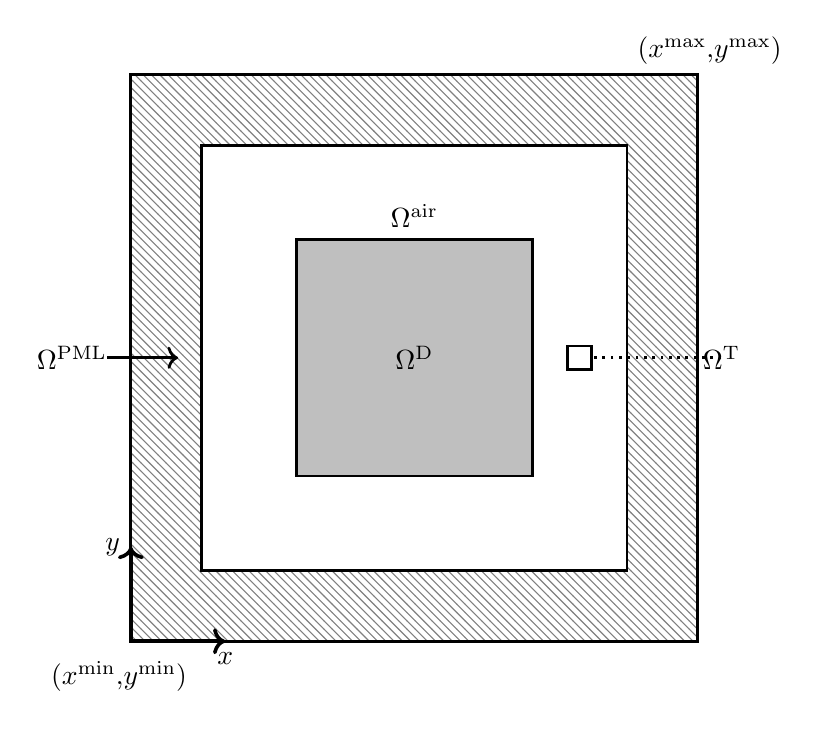
\begin{tikzpicture}[scale=3.0, line width = 1.0pt]
			
			\draw[pattern=north west lines, pattern color=gray] (-1.2,-1.2) rectangle (1.2,1.2);
			\draw[fill = white] (-0.9,-0.9) rectangle (0.9,0.9);
			\draw[fill=lightgray] (-0.5,-0.5) rectangle (0.5,0.5);
			\draw[black] (0.65,-0.05) rectangle (0.75,0.05);
			\draw[black] (1.3,0) node {$\Omega^\text{T}$};
			\draw[dotted] (1.3,0) -- (0.75,0.0); 
			\draw[black] (0,0) node {$\Omega^\text{D}$};
			\draw[black] (0,0.6) node {$\Omega^\text{air}$};
			\draw[black] (-1.45,0) node {$\Omega^\text{PML}$};
			\draw[->] (-1.3,0) -- (-1,0);
			
			\draw[black,line width=1.3pt, ->] (-1.2,-1.2) -- (-1.2,-0.8) node[left] {$y$}; 
			\draw[black,line width=1.3pt, ->] (-1.2,-1.2) -- (-0.8,-1.2) node[below] {$x$}; 
			
			\draw[black]  (-1.25,-1.35) node {($x^\text{min}$,$y^\text{min}$)};
			
			 \draw[black]  (1.25,1.3) node {($x^\text{max}$,$y^\text{max}$)};
			
			
	\end{tikzpicture}
	\endpgfgraphicnamed
\end{document}